% Options for packages loaded elsewhere
\PassOptionsToPackage{unicode}{hyperref}
\PassOptionsToPackage{hyphens}{url}
\PassOptionsToPackage{dvipsnames,svgnames,x11names}{xcolor}
%
\documentclass[
  12pt,
  a4paper,
]{article}

\usepackage{amsmath,amssymb}
\usepackage{setspace}
\usepackage{iftex}
\ifPDFTeX
  \usepackage[T1]{fontenc}
  \usepackage[utf8]{inputenc}
  \usepackage{textcomp} % provide euro and other symbols
\else % if luatex or xetex
  \usepackage{unicode-math}
  \defaultfontfeatures{Scale=MatchLowercase}
  \defaultfontfeatures[\rmfamily]{Ligatures=TeX,Scale=1}
\fi
\usepackage{lmodern}
\ifPDFTeX\else  
    % xetex/luatex font selection
    \setmainfont[]{Latin Modern Roman}
    \setsansfont[]{Latin Modern Roman}
\fi
% Use upquote if available, for straight quotes in verbatim environments
\IfFileExists{upquote.sty}{\usepackage{upquote}}{}
\IfFileExists{microtype.sty}{% use microtype if available
  \usepackage[]{microtype}
  \UseMicrotypeSet[protrusion]{basicmath} % disable protrusion for tt fonts
}{}
\usepackage{xcolor}
\usepackage[top=2.5cm,bottom=2.5cm,left=2.5cm,right=2.5cm]{geometry}
\setlength{\emergencystretch}{3em} % prevent overfull lines
\setcounter{secnumdepth}{5}
% Make \paragraph and \subparagraph free-standing
\makeatletter
\ifx\paragraph\undefined\else
  \let\oldparagraph\paragraph
  \renewcommand{\paragraph}{
    \@ifstar
      \xxxParagraphStar
      \xxxParagraphNoStar
  }
  \newcommand{\xxxParagraphStar}[1]{\oldparagraph*{#1}\mbox{}}
  \newcommand{\xxxParagraphNoStar}[1]{\oldparagraph{#1}\mbox{}}
\fi
\ifx\subparagraph\undefined\else
  \let\oldsubparagraph\subparagraph
  \renewcommand{\subparagraph}{
    \@ifstar
      \xxxSubParagraphStar
      \xxxSubParagraphNoStar
  }
  \newcommand{\xxxSubParagraphStar}[1]{\oldsubparagraph*{#1}\mbox{}}
  \newcommand{\xxxSubParagraphNoStar}[1]{\oldsubparagraph{#1}\mbox{}}
\fi
\makeatother


\providecommand{\tightlist}{%
  \setlength{\itemsep}{0pt}\setlength{\parskip}{0pt}}\usepackage{longtable,booktabs,array}
\usepackage{calc} % for calculating minipage widths
% Correct order of tables after \paragraph or \subparagraph
\usepackage{etoolbox}
\makeatletter
\patchcmd\longtable{\par}{\if@noskipsec\mbox{}\fi\par}{}{}
\makeatother
% Allow footnotes in longtable head/foot
\IfFileExists{footnotehyper.sty}{\usepackage{footnotehyper}}{\usepackage{footnote}}
\makesavenoteenv{longtable}
\usepackage{graphicx}
\makeatletter
\def\maxwidth{\ifdim\Gin@nat@width>\linewidth\linewidth\else\Gin@nat@width\fi}
\def\maxheight{\ifdim\Gin@nat@height>\textheight\textheight\else\Gin@nat@height\fi}
\makeatother
% Scale images if necessary, so that they will not overflow the page
% margins by default, and it is still possible to overwrite the defaults
% using explicit options in \includegraphics[width, height, ...]{}
\setkeys{Gin}{width=\maxwidth,height=\maxheight,keepaspectratio}
% Set default figure placement to htbp
\makeatletter
\def\fps@figure{htbp}
\makeatother
% definitions for citeproc citations
\NewDocumentCommand\citeproctext{}{}
\NewDocumentCommand\citeproc{mm}{%
  \begingroup\def\citeproctext{#2}\cite{#1}\endgroup}
\makeatletter
 % allow citations to break across lines
 \let\@cite@ofmt\@firstofone
 % avoid brackets around text for \cite:
 \def\@biblabel#1{}
 \def\@cite#1#2{{#1\if@tempswa , #2\fi}}
\makeatother
\newlength{\cslhangindent}
\setlength{\cslhangindent}{1.5em}
\newlength{\csllabelwidth}
\setlength{\csllabelwidth}{3em}
\newenvironment{CSLReferences}[2] % #1 hanging-indent, #2 entry-spacing
 {\begin{list}{}{%
  \setlength{\itemindent}{0pt}
  \setlength{\leftmargin}{0pt}
  \setlength{\parsep}{0pt}
  % turn on hanging indent if param 1 is 1
  \ifodd #1
   \setlength{\leftmargin}{\cslhangindent}
   \setlength{\itemindent}{-1\cslhangindent}
  \fi
  % set entry spacing
  \setlength{\itemsep}{#2\baselineskip}}}
 {\end{list}}
\usepackage{calc}
\newcommand{\CSLBlock}[1]{\hfill\break\parbox[t]{\linewidth}{\strut\ignorespaces#1\strut}}
\newcommand{\CSLLeftMargin}[1]{\parbox[t]{\csllabelwidth}{\strut#1\strut}}
\newcommand{\CSLRightInline}[1]{\parbox[t]{\linewidth - \csllabelwidth}{\strut#1\strut}}
\newcommand{\CSLIndent}[1]{\hspace{\cslhangindent}#1}

\usepackage{booktabs}
\usepackage{longtable}
\usepackage{array}
\usepackage{multirow}
\usepackage{wrapfig}
\usepackage{float}
\usepackage{colortbl}
\usepackage{pdflscape}
\usepackage{tabu}
\usepackage{threeparttable}
\usepackage{threeparttablex}
\usepackage[normalem]{ulem}
\usepackage{makecell}
\usepackage{xcolor}
\usepackage{fancyhdr}
\usepackage{amsmath}
\usepackage{multirow}
\usepackage{booktabs}
\makeatletter
\@ifpackageloaded{caption}{}{\usepackage{caption}}
\AtBeginDocument{%
\ifdefined\contentsname
  \renewcommand*\contentsname{Table of contents}
\else
  \newcommand\contentsname{Table of contents}
\fi
\ifdefined\listfigurename
  \renewcommand*\listfigurename{List of Figures}
\else
  \newcommand\listfigurename{List of Figures}
\fi
\ifdefined\listtablename
  \renewcommand*\listtablename{List of Tables}
\else
  \newcommand\listtablename{List of Tables}
\fi
\ifdefined\figurename
  \renewcommand*\figurename{Figure}
\else
  \newcommand\figurename{Figure}
\fi
\ifdefined\tablename
  \renewcommand*\tablename{Table}
\else
  \newcommand\tablename{Table}
\fi
}
\@ifpackageloaded{float}{}{\usepackage{float}}
\floatstyle{ruled}
\@ifundefined{c@chapter}{\newfloat{codelisting}{h}{lop}}{\newfloat{codelisting}{h}{lop}[chapter]}
\floatname{codelisting}{Listing}
\newcommand*\listoflistings{\listof{codelisting}{List of Listings}}
\makeatother
\makeatletter
\makeatother
\makeatletter
\@ifpackageloaded{caption}{}{\usepackage{caption}}
\@ifpackageloaded{subcaption}{}{\usepackage{subcaption}}
\makeatother

\ifLuaTeX
  \usepackage{selnolig}  % disable illegal ligatures
\fi
\usepackage{bookmark}

\IfFileExists{xurl.sty}{\usepackage{xurl}}{} % add URL line breaks if available
\urlstyle{same} % disable monospaced font for URLs
\hypersetup{
  pdftitle={Estimation of Effects of Endogenous Time-Varying Covariates: A Comparison Of Multilevel Linear Modeling and Generalized Estimating Equations},
  pdfauthor={Ward B. Eiling (9294163)},
  colorlinks=true,
  linkcolor={blue},
  filecolor={Maroon},
  citecolor={Blue},
  urlcolor={Blue},
  pdfcreator={LaTeX via pandoc}}


\title{Estimation of Effects of Endogenous Time-Varying Covariates: A
Comparison Of Multilevel Linear Modeling and Generalized Estimating
Equations}
\usepackage{etoolbox}
\makeatletter
\providecommand{\subtitle}[1]{% add subtitle to \maketitle
  \apptocmd{\@title}{\par {\large #1 \par}}{}{}
}
\makeatother
\subtitle{Research Report}
\author{Ward B. Eiling (9294163)}
\date{December 22, 2024}

\begin{document}
\cleardoublepage
\thispagestyle{empty}
{\centering
\hbox{}\vskip 0cm plus 1fill
% \vspace{25ex}
{\Large\bfseries Estimation of Effects of Endogenous Time-Varying
Covariates: A Comparison Of Multilevel Linear Modeling and Generalized
Estimating Equations \par}
\vspace{3ex}
{\large Research Report \par}
\vspace{9ex}
{\large\bfseries Ward B. Eiling (9294163) \par}
\vspace{3ex}
% {\Large ORCID: 0009-0007-8114-9497 \par}
% \vspace{3ex}
{\large Supervisors: Ellen Hamaker and Jeroen Mulder \par}
% \vskip 0cm plus 2fill
\vspace{9ex}
{\normalsize \textit{Master's degree in Methodology and Statistics for the Behavioural, \\ Biomedical and Social Sciences} \par}
\vspace{3ex}
{\normalsize \textit{Utrecht University} \par}
\vspace{9ex}
{\normalsize December 22, 2024 \par}
\vspace{3ex}
{\normalsize Word count: 728 \par}
\vspace{9ex}
{\normalsize FETC-approved: 24-2003 \par}
\vspace{9ex}
{\normalsize \textit{Candidate journal: Psychological Methods} \par}
\hbox{}\vskip 0cm plus 1fill
% \vspace{12ex}
% %
% %
% {\large Utrecht University \par}
% %
% %
% {\large Methodology and Statistics \par}
% \vspace{3ex}
% %
% {\large  \par}
% %
% \vspace{12ex}
% {\small Submitted in total fulfilment of the requirements
% of the degree of Doctor of Philosophy \par}
}


\setstretch{2}
\newpage

\section{Introduction}\label{introduction}

Across a wide range of disciplines, researchers analyze clustered
longitudinal, observational data to investigate prospective causal
relationships between variables. When analyzing such data, the
psychological sciences most commonly resort to the multilevel linear
model (MLM, \citeproc{ref-mcneish2017}{McNeish et al., 2017}),
which---in the context of longitudinal data analysis---separates
observed variance into stable between-person differences and
within-person fluctuations (\citeproc{ref-hamaker2020}{Hamaker \&
Muthén, 2020}). Conversely, other fields, such as biostatistics and
econometrics often favour generalized estimating equations (GEE) for the
analysis of longitudinal data (\citeproc{ref-mcneish2017}{McNeish et
al., 2017}). Despite some cross-disciplinary efforts to compare these
methods (\citeproc{ref-mcneish2017}{McNeish et al., 2017};
\citeproc{ref-muth2016}{Muth et al., 2016}; \citeproc{ref-yan2013}{Yan
et al., 2013}), their scarcity may leave researchers with limited
guidance in choosing the most suitable approach for their application.

A recent study by Qian et al. (\citeproc{ref-qian2020}{2020})
highlighted an issue present in both methods---except for GEE with
working independence---where controlling for \emph{time-varying
endogenous covariates} may lead to biased causal estimates. A
time-varying covariate is \emph{endogenous} if it is directly or
indirectly influenced by prior treatment or outcome, meaning its value
may be determined by earlier stages of the process
(\citeproc{ref-qian2020}{Qian et al., 2020}).
Figure~\ref{fig-endogenous-example} showcases a time-varying endogenous
covariate \(X_{it}\) in the context of a simple multilevel linear model
with a random intercept \(b_{0i}\). As a result of including these
covariates in these models, ordinary interpretations of the coefficients
are no longer valid (\citeproc{ref-qian2020}{Qian et al., 2020, p. 3}).
According to Diggle (\citeproc{ref-diggle2002}{2002}), this issue not
only pertains GEE and MLM, but \emph{all} longitudinal data analysis
methods.

\begin{figure}[H]

\caption{\label{fig-endogenous-example}Multilevel Linear Model with
Time-Varying Endogenous Covariate \(X_{it}\).}

\centering{

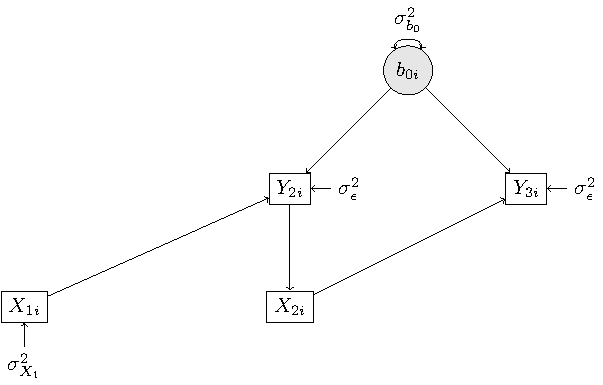
\includegraphics{research-report_files/figure-pdf/endogenous-example-1.pdf}

\emph{Note}. Adapted from Section 2.2 of Qian et al.
(\citeproc{ref-qian2020}{2020}).

}

\end{figure}%

However, due to a divide between the disciplines that employ these
methods, such critiques of the MLM appear to have largely failed to
reach the applied researcher in psychology. One specific reason might be
that the technical jargon in other disciplines makes it difficult for
researchers to recognize when and how these issues emerge{[}\^{}1{]}.
Therefore, this report aims to understand and explain the issue of
including endogenous covariates in analyses involving GEE and MLM in a
psychological context. To achieve this aim, the current investigation
employs (a) graphical tools such as the directed acyclic graph (DAG) and
path diagram to assess potentially relevant assumptions, as well as (b)
data simulations with additional scenarios to pinpoint the issue.
Accordingly, the following research questions will be addressed:

\begin{enumerate}
\def\labelenumi{(\arabic{enumi})}
\item
  When does the inclusion of endogenous variables in multilevel linear
  models result in biased estimates of the treatment effect?
\item
  When does the inclusion of of endogenous covariates in multilevel
  linear models result in a discrepancy between conditional and marginal
  interpretations of the treatment effect?
\end{enumerate}

\section{Methods}\label{methods}

To obtain a better understanding of the issue exposed by Qian et al.
(\citeproc{ref-qian2020}{2020}), two methods were employed. First,
graphical methods were used provide insight into the presence and extent
of bias with potential violation of assumptions: (a) path diagrams were
used to evaluate the conditional independence assumption and (b)
directed acyclic graphs (DAGs) were used to evaluate the backdoor
criterion (Pearl, 1988, 2009). Second, a simulation study was performed
to reproduce the results for the generative models (GMs) from Qian et
al. (\citeproc{ref-qian2020}{2020}) and to further isolate the issue
using additional GMs. In this simulation, bias in the treatment effect
(RQ 1) was assessed with analytical multilevel models. The discrepancy
between conditional and marginal interpretations of the treatment effect
(RQ 2) was assessed with GEE with working independence.

\subsection{Data Generation}\label{data-generation}

In the simulation Qian et al. (\citeproc{ref-qian2020}{2020}) considered
three generative models (GMs), all of which have an endogenous
time-varying covariate. In GM1 and GM2, the endogenous covariate
\(X_{it}\) equals the previous outcome \(Y_{it}\) plus some random
noise, so the \emph{conditional independence} assumption is valid. In
GM3, the endogenous covariate depends directly on \(b_{i0}\), violating
the assumption. To isolate the issue in GM3, we consider two variations
on this model: GM3A, where the random slope \(b_{i2}\) for the treatment
\(A_{it}\) is removed; GM3B, where the interaction term
\(\beta_1 A_{it} X_{it}\) is removed. Note that the conditional
independence assumption is violated in either of these variations. The
details of the generative models are described below. We follow the
notation of Qian et al. (\citeproc{ref-qian2020}{2020}) to allow for
direct comparison, but rewrite the equations into within- and
between-person models (see \citeproc{ref-raudenbush2002}{Raudenbush \&
Bryk, 2002}). We accompany the equations of the GMs with graphical
representations, where random effects are represented by grey circles,
observed variables by squares and relationships across variables by
arrows. The path diagrams of the three data generating models shows the
discrepancies between the different generative models---especially
concerning the interaction effects---more clearly than DAGs.

\subsubsection{Generative Model 1}\label{generative-model-1}

In GM1, we considered a simple case with only a random intercept and a
random slope for \(X_{it}\). The outcome is generated according to the
following repeated-observations or within-person model (level 1):

\[
Y_{it+1} = \pi_{0i} + \pi_{1i} X_{it} + \pi_{2i} A_{it} + \pi_{3i} A_{it} X_{it} + \epsilon_{it+1}
\]

with the person-level or between-person model (level 2):

\[
\pi_{0i} = \alpha_0 + b_{i0}, \quad b_{i0} \sim \mathcal{N}(0, \sigma_{b0}^2),
\]

\[
\pi_{1i} = \alpha_1,
\]

\[
\pi_{2i} = \beta_0 + b_{i2}, \quad b_{i2} \sim \mathcal{N}(0, \sigma_{b2}^2),
\]

\[
\pi_{3i} = \beta_1.
\]

By substitution, we get the single equation model:

\[
\begin{aligned}
Y_{it+1} &= \pi_{0i} + \pi_{1i} X_{it} + \pi_{2i} A_{it} + \pi_{3i} A_{it} X_{it} + \epsilon_{it+1} \\
&= (\alpha_0 + b_{i0}) + \alpha_1 X_{it} + (\beta_0 + b_{i2}) A_{it} + \beta_1 A_{it} X_{it} + \epsilon_{it+1} \\
&= \alpha_0 + \alpha_1 X_{it} + b_{i0} + A_{it} (\beta_0 + \beta_1 X_{it} + b_{i2}) + \epsilon_{it+1}.
\end{aligned}
\]

The random effects \(b_{i0} \sim \mathcal{N}(0, \sigma_{b0}^2)\) and
\(b_{i2} \sim \mathcal{N}(0, \sigma_{b2}^2)\) are independent of each
other. The covariate is generated as \(X_{i1} \sim \mathcal{N}(0, 1)\),
and for \(t \geq 2\),

\[
X_{it} = Y_{it} + \mathcal{N}(0, 1).
\]

The randomization probability \(p_t = P(A_{it} = 1 \mid H_{it})\) is
constant at \(1/2\). Thus, \(A_{it} \sim \text{Bernoulli}(0.5)\) for
\(i = 1, \ldots, N\) and \(t = 1, \ldots, T\). The exogenous noise is
\(\epsilon_{it+1} \sim \mathcal{N}(0, \sigma_\epsilon^2)\).

Figure~\ref{fig-GM1_path} shows the path diagram for GM1.

\begin{figure}[H]

\caption{\label{fig-GM1_path}Path diagram for Generative Model 1
(\(t = 1, 2, 3\))}

\centering{

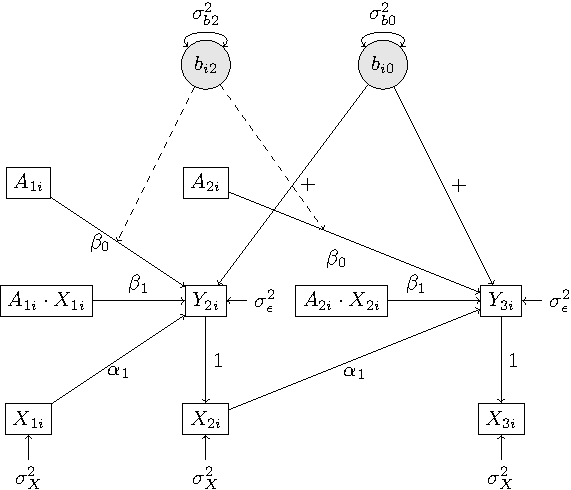
\includegraphics{research-report_files/figure-pdf/fig-GM1_path-1.pdf}

}

\end{figure}%

\subsubsection{Generative Model 2}\label{generative-model-2}

In GM2, we considered the case with a random intercept and random slopes
for (1) covariate \(X_{it}\), (2) treatment \(A_{it}\), and (3) the
interaction between \(A_{it}\) and \(X_{it}\); and with a time-varying
randomization probability for treatment. The outcome is generated
according to the same repeated-observations model presented in GM1.
However, the person-level model is different:

\[
\pi_{0i} = \alpha_0 + b_{i0}, \quad b_{i0} \sim \mathcal{N}(0, \sigma_{b0}^2),
\]

\[
\pi_{1i} = \alpha_1 + b_{i1}, \quad b_{i1} \sim \mathcal{N}(0, \sigma_{b1}^2),
\]

\[
\pi_{2i} = \beta_0 + b_{i2}, \quad b_{i2} \sim \mathcal{N}(0, \sigma_{b2}^2),
\]

\[
\pi_{3i} = \beta_1 + b_{i3}, \quad b_{i3} \sim \mathcal{N}(0, \sigma_{b3}^2).
\]

By substitution, we get the single equation model:

\[
\begin{aligned}
Y_{it+1} &= \pi_{0i} + \pi_{1i} X_{it} + \pi_{2i} A_{it} + \pi_{3i} A_{it} X_{it} + \epsilon_{it+1} \\ 
&= (\alpha_0 + b_{i0}) + (\alpha_1 + b_{i1}) X_{it} + (\beta_0 + b_{i2}) A_{it} + (\beta_1 + b_{i3}) A_{it} X_{it} + \epsilon_{it+1} \\ 
&= \alpha_0 + \alpha_1 X_{it} + b_{i0} + b_{i1} X_{it} + A_{it} \left( \beta_0 + \beta_1 X_{it} + b_{i2} + b_{i3} X_{it} \right) + \epsilon_{it+1}.
\end{aligned}
\]

The random effects \(b_{ij} \sim \mathcal{N}(0, \sigma_{bj}^2)\), for
\(j = 0, 1, 2, 3\), are independent of each other. The covariate is
generated as \(X_{i1} \sim \mathcal{N}(0, 1)\), and for \(t \geq 2\),

\[
X_{it} = Y_{it} + \mathcal{N}(0, 1).
\]

The randomization probability depends on \(X_{it}\):

\[
p_t = P(A_{it} = 1 \mid H_{it}) = 
\begin{cases} 
0.7 & \text{if } X_{it} > -1.27, \\
0.3 & \text{if } X_{it} \leq -1.27,
\end{cases}
\]

where the cutoff \(-1.27\) was chosen so that \(p_t\) equals 0.7 or 0.3
for about half of the time. In other words, if the value of the
covariate for any given person and time point is above the cutoff, the
probability of receiving the treatment \(p_t\) is 0.7; otherwise, it is
0.3. Accordingly, \(A_{it} \sim \text{Bernoulli}(p_t)\) for
\(i = 1, \ldots, N\) and \(t = 1, \ldots, T\). The exogenous noise is
\(\epsilon_{it+1} \sim \mathcal{N}(0, \sigma_\epsilon^2)\).

Figure~\ref{fig-GM2_path} shows the path diagram for GM2.

\begin{figure}[H]

\caption{\label{fig-GM2_path}Path diagram for Generative Model 2
(\(t = 1, 2, 3\))}

\centering{

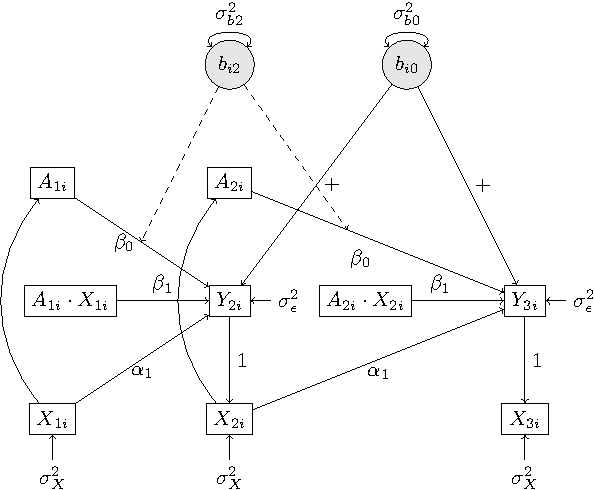
\includegraphics{research-report_files/figure-pdf/fig-GM2_path-1.pdf}

}

\end{figure}%

\subsubsection{Generative Model 3}\label{generative-model-3}

GM3 is the same as GM1, except that the covariate \(X_{it}\) depends
directly on \(b_{i0}\):

\[
X_{i1} \sim \mathcal{N}(b_{i0}, 1), \quad X_{it} = Y_{it} + \mathcal{N}(b_{i0}, 1) \text{ for } t \geq 2.
\]

Figure~\ref{fig-GM3_path} shows the path diagram for GM3.

\begin{figure}[H]

\caption{\label{fig-GM3_path}Path diagram for Generative Model 3
(\(t = 1, 2, 3\))}

\centering{

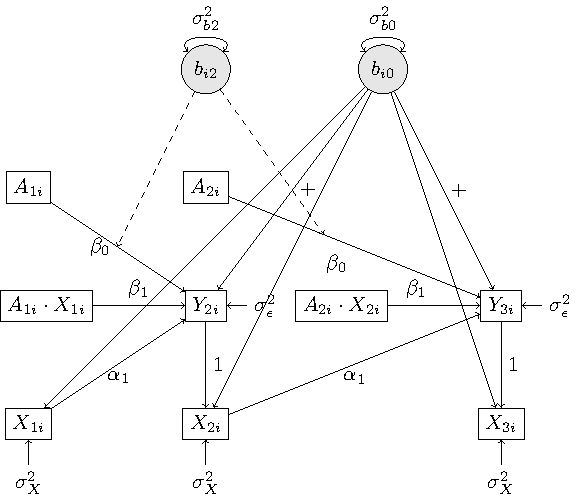
\includegraphics{research-report_files/figure-pdf/fig-GM3_path-1.pdf}

}

\end{figure}%

\subsubsection{Generative Model 3A}\label{generative-model-3a}

GM3A is the same as GM3, except that the random slope \(b_{i2}\) for the
treatment \(A_{it}\) is removed. The single equation model then becomes:

\[
Y_{it+1} = \alpha_0 + \alpha_1 X_{it} + b_{i0} + A_{it} (\beta_0 + \beta_1 X_{it}) + \epsilon_{it+1}.
\]

\begin{figure}[H]

\caption{\label{fig-GM3A_path}Path diagram for Generative Model 3A
(\(t = 1, 2, 3\))}

\centering{

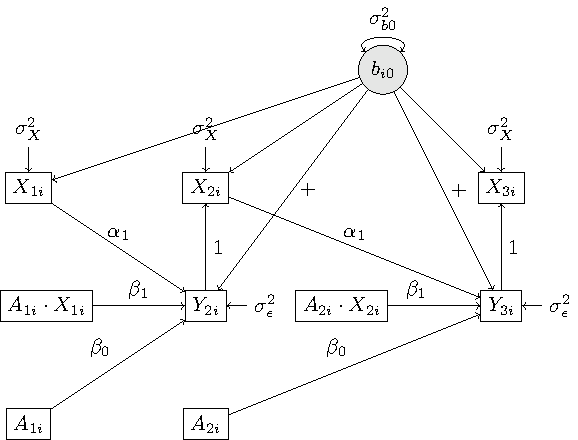
\includegraphics{research-report_files/figure-pdf/fig-GM3A_path-1.pdf}

}

\end{figure}%

\subsubsection{Generative Model 3B}\label{generative-model-3b}

GM3B is the same as GM3, except that the interaction term
\(\beta_1 A_{it} X_{it}\) is removed. The single equation model then
becomes:

\[
Y_{it+1} = \alpha_0 + \alpha_1 X_{it} + b_{i0} + A_{it} (\beta_0 + b_{i2}) + \epsilon_{it+1}.
\]

\begin{figure}[H]

\caption{\label{fig-GM3B_path}Path diagram for Generative Model 3B
(\(t = 1, 2, 3\))}

\centering{

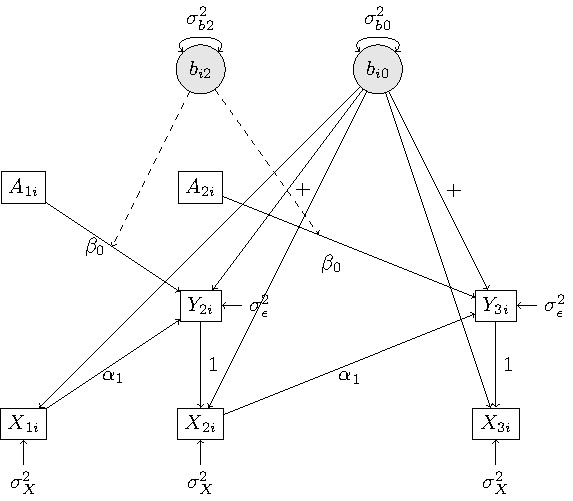
\includegraphics{research-report_files/figure-pdf/fig-GM3B_path-1.pdf}

}

\end{figure}%

\subsubsection{Parameter Values}\label{parameter-values}

The following parameter values were adapted from Qian et al.
(\citeproc{ref-qian2020}{2020}):

\[
\alpha_0 = -2, \quad \alpha_1 = -0.3, \quad \beta_0 = 1, \quad \beta_1 = 0.3,
\]

\[
\sigma_{b0}^2 = 4, \quad \sigma_{b1}^2 = \frac{1}{4}, \quad \sigma_{b2}^2 = 1, \quad \sigma_{b3}^2 = \frac{1}{4}, \quad \sigma_\epsilon^2 = 1.
\]

\subsection{Path Diagrams and Conditional
Independence}\label{path-diagrams-and-conditional-independence}

Qian et al. (\citeproc{ref-qian2020}{2020}) proposes the use of the
conditional independence assumption to identify whether bias may occur,
which is given by:

\[ X_{it} \perp (b_{i0}, b_{i1}) \mid H_{it-1}, A_{it-1}, Y_{it}. \]

where \(H_{it-1}\) refers to the history of the set of covariates, which
in this case are all observations of covariate \(X_{it}\) prior to the
current timepoint \(t\). This allows \(X_{it}\) to be endogenous, but
the endogenous covariate \(X_{it}\) can only depend on the random
effects through variables observed prior to \(X_{it}\). If the only
endogenous covariates are functions of prior treatments and prior
outcomes, then the assumption automatically holds.

When inspecting Figure~\ref{fig-GM1_path} and Figure~\ref{fig-GM2_path},
we may notice that \(X_{it}\) becomes independent of the random effects
after conditioning on \(Y_{it}\). On the other hand, we can see that
this assumption is violated in GM3/3A/3B, as \(X_{it}\) depends directly
on \(b_{i0}\) and can thus not be made independent of the random effects
by conditioning on prior variables such as \(Y_{it}\) (see
Figure~\ref{fig-GM3_path}, Figure~\ref{fig-GM3A_path} and
Figure~\ref{fig-GM3B_path}). Thus, we would expect biased estimates of
the treatment effect for GM3/3A/3B.

\subsection{Backdoor Criterion and
DAGs}\label{backdoor-criterion-and-dags}

DAGs are a useful tool for representing causal relationships between
variables and to evaluate the assumptions needed for causal
identification. According to the backdoor criterion
(\citeproc{ref-pearl1988}{Pearl, 1988}, \citeproc{ref-pearl2009}{2009}),
a requirement for causal identification, causal effects can be
identified by blocking non-causal paths through conditioning on
intermediate variables (e.g., controlling or matching). If any
non-causal paths cannot be blocked due to omitted variables or
measurement error, treatment and outcome remain linked via backdoor
paths, leading to biased estimates of the treatment effect
(\citeproc{ref-Kim2021a}{Kim \& Steiner, 2021}).

We formulated the DAGs in \texttt{dagitty}, where the random disturbance
\(b_{0i}\) was represented by the node U (e.g.,
\citeproc{ref-Kim2021a}{Kim \& Steiner, 2021}). The DAGs for the first
three observations of the three data generating models are presented in
Figure~\ref{fig-DAGs}.

\begin{figure}[H]

\caption{\label{fig-DAGs}DAGs for Generative Models 1, 2, 3, 3A, 3B (t =
1, 2, 3)}

\begin{minipage}{0.50\linewidth}

\subcaption{\label{fig-GM1_DAG}GM 1}

\centering{

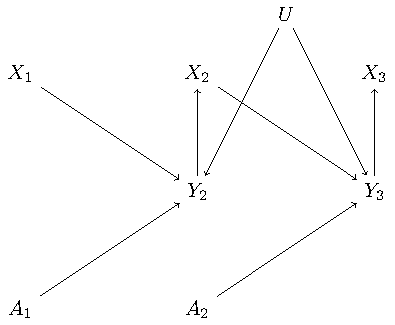
\includegraphics{research-report_files/figure-pdf/fig-GM1_DAG-1.pdf}

}

\end{minipage}%
%
\begin{minipage}{0.50\linewidth}

\subcaption{\label{fig-GM2_DAG}GM 2}

\centering{

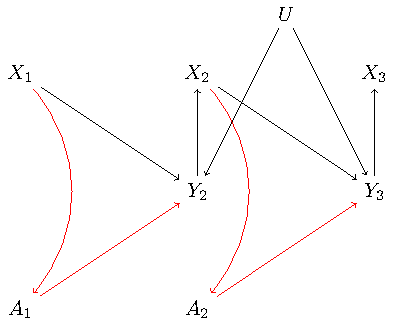
\includegraphics{research-report_files/figure-pdf/fig-GM2_DAG-1.pdf}

}

\end{minipage}%
\newline
\begin{minipage}{0.50\linewidth}

\subcaption{\label{fig-GM3_DAG}GM 3, 3A, 3B}

\centering{

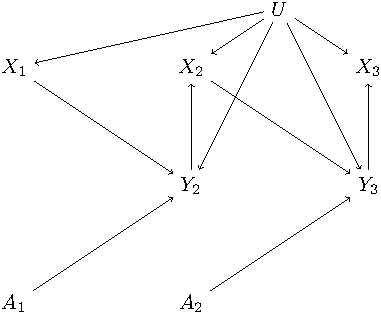
\includegraphics{research-report_files/figure-pdf/fig-GM3_DAG-1.pdf}

}

\end{minipage}%
%
\begin{minipage}{0.50\linewidth}
\emph{Note.} The red arrows show the biased backdoor path(s) in the
treatment efffect (before controlling for \(X_{it}\)).\end{minipage}%

\end{figure}%

When applying Pearl's backdoor criterion to GM1/3/3A/3B, it may be
observed that there exists no backdoor path in the treatment effect
\(A_{it} \to Y_{it+1}\), as \(A_{it}\) does not have any parents. While
we need not control for covariate \(X_{it}\) to obtain an unbiased total
effect, doing so should not introduce bias.

On the other hand, in GM2, there is a backdoor path in the treatment
effect: \(A_{it} \leftarrow X_{it} \rightarrow Y_{it+1}\) (see
Figure~\ref{fig-GM2_DAG}). More specifically, \(X_{it}\) is a confounder
in the relationship between \(A_{it}\) and \(Y_{it+1}\). However,
controlling for \(X_{it}\) blocks this backdoor path, making the
treatment effect unbiased. In other words, the history of covariate
\(X_{it}\) is a sufficient adjustment set for the treatment effect.

All things considered, according to the backdoor criterion, controlling
for the covariate \(X_{it}\) should not result in biased estimates of
the treatment effect for any of the generative models.

\subsection{Data Analysis}\label{data-analysis}

We evaluated the performance of the models across a total of 30
different settings, each replicated 1,000 times, by systematically
varying the following factors:

\begin{itemize}
\item
  \textbf{Generative Models (GM):} 1, 2, 3, 3A, 3B
\item
  \textbf{Number of timepoints (T):} 10, 30
\item
  \textbf{Sample size (N):} 30, 100, 200
\end{itemize}

All data generation and estimation was performed in \texttt{R}, version
4.4.2 (\citeproc{ref-rcoreteam2024}{Team, 2024}). After the generation
of data generation for any given setting, several models were fit. To
fit the standard MLM, the \texttt{lmer} function from the R-package
\texttt{lme4} (\citeproc{ref-bates2015}{Bates et al., 2015}) was
employed with restricted maximum likelihood estimation. For the MLM, the
analytical models were equivalent to each of the respective
data-generating models. To fit the GEE with the ``exchangeable'',
``independent'' and ``AR(1)'' working correlation structures, the
\texttt{geeglm} function from the R-package \texttt{geepack}
(\citeproc{ref-halekoh2006}{Halekoh et al., 2006}) was employed with the
identity link function. Since the random effects are not explicitly
modelled in GEE, the analytical GEE models simply contain only the fixed
effects of the generative model at hand.

\section{Results}\label{results}

Table~\ref{tbl-simulation-results} presents the simulation results for
each of the generative and analytical models. The estimates for the
analytical MLM may be interpreted in terms of bias. Here we find that
there is little to no bias for GM1/2/3A/3B and substantial bias for GM3.
Thus, once we remove either the dependency of the random intercept with
the covariate (GM1), the random slope \(b_{i2}\) (GM3A) or the
interaction \(\beta_1\) (GM3B) from GM3, the bias dissapears or becomes
extremely small. The bias in GM3 decreases as the number of timepoints
\(T\) increases from 10 to 30. Note that the MLM model fitting success
rates are particularly poor for GM2, where in the worst case, only 87 of
the 1000 models were fitted.

For the GEE with independence, the values refer to the difference
between the estimated marginal effect---which should be unbiased under
endogenous covariates (see \citeproc{ref-pepe1994}{Pepe \& Anderson,
1994})---and the specified conditional effect. Here we find that there
is a enormous difference between these effects for GM2, which increases
along with an increase in \(T\) and \(N\), up to a difference of more
than 6,000. This is followed by a difference of around .07-.09 for GM1,
.02-.04 for GM3, \(\leq 0.015\) for GM3B and close to zero for GM3A. The
GEE models fitted succesfully for all settings.

\begin{table}

\caption{\label{tbl-simulation-results}Simulation results for Generative
Models 1, 2, 3, 3A and 3B over 1000 replications}

\centering{

\centering\centering
\begin{tabular}[t]{>{\raggedright\arraybackslash}p{5em}rrrrrrrr}
\toprule
\multicolumn{3}{c}{ } & \multicolumn{3}{c}{MLM} & \multicolumn{3}{c}{GEE-IND} \\
\cmidrule(l{3pt}r{3pt}){4-6} \cmidrule(l{3pt}r{3pt}){7-9}
GM & T & N & Bias & SD & SR & Difference & SD & SR\\
\midrule
 &  & 30 & 0.000 & 0.238 & 0.998 & 0.071 & 0.296 & 1\\
\cmidrule{3-9}
 &  & 100 & -0.012 & 0.129 & 1.000 & 0.074 & 0.169 & 1\\
\cmidrule{3-9}
 & \multirow{-3}{*}{\raggedleft\arraybackslash 10} & 200 & 0.003 & 0.093 & 0.999 & 0.085 & 0.116 & 1\\
\cmidrule{2-9}
 &  & 30 & -0.001 & 0.203 & 0.998 & 0.085 & 0.224 & 1\\
\cmidrule{3-9}
 &  & 100 & -0.007 & 0.107 & 0.996 & 0.083 & 0.123 & 1\\
\cmidrule{3-9}
\multirow{-6}{5em}[0.5\dimexpr\aboverulesep+\belowrulesep+\cmidrulewidth]{\raggedright\arraybackslash 1} & \multirow{-3}{*}{\raggedleft\arraybackslash 30} & 200 & 0.001 & 0.079 & 0.996 & 0.094 & 0.088 & 1\\
\cmidrule{1-9}
 &  & 30 & 0.011 & 0.282 & 0.925 & 0.306 & 1.630 & 1\\
\cmidrule{3-9}
 &  & 100 & 0.005 & 0.147 & 0.881 & 0.565 & 1.836 & 1\\
\cmidrule{3-9}
 & \multirow{-3}{*}{\raggedleft\arraybackslash 10} & 200 & 0.008 & 0.103 & 0.844 & 0.935 & 1.887 & 1\\
\cmidrule{2-9}
 &  & 30 & 0.000 & 0.220 & 0.603 & 182.565 & 4751.387 & 1\\
\cmidrule{3-9}
 &  & 100 & -0.014 & 0.114 & 0.247 & -356.412 & 39799.388 & 1\\
\cmidrule{3-9}
\multirow{-6}{5em}[0.5\dimexpr\aboverulesep+\belowrulesep+\cmidrulewidth]{\raggedright\arraybackslash 2} & \multirow{-3}{*}{\raggedleft\arraybackslash 30} & 200 & -0.013 & 0.087 & 0.087 & 6319.792 & 136201.790 & 1\\
\cmidrule{1-9}
 &  & 30 & -0.052 & 0.245 & 0.999 & 0.020 & 0.249 & 1\\
\cmidrule{3-9}
 &  & 100 & -0.064 & 0.134 & 1.000 & 0.024 & 0.141 & 1\\
\cmidrule{3-9}
 & \multirow{-3}{*}{\raggedleft\arraybackslash 10} & 200 & -0.051 & 0.096 & 1.000 & 0.035 & 0.097 & 1\\
\cmidrule{2-9}
 &  & 30 & -0.024 & 0.206 & 0.997 & 0.030 & 0.208 & 1\\
\cmidrule{3-9}
 &  & 100 & -0.030 & 0.108 & 0.996 & 0.027 & 0.112 & 1\\
\cmidrule{3-9}
\multirow{-6}{5em}[0.5\dimexpr\aboverulesep+\belowrulesep+\cmidrulewidth]{\raggedright\arraybackslash 3} & \multirow{-3}{*}{\raggedleft\arraybackslash 30} & 200 & -0.023 & 0.080 & 0.997 & 0.037 & 0.081 & 1\\
\cmidrule{1-9}
 &  & 30 & 0.000 & 0.126 & 1.000 & -0.004 & 0.157 & 1\\
\cmidrule{3-9}
 &  & 100 & 0.004 & 0.073 & 1.000 & 0.001 & 0.090 & 1\\
\cmidrule{3-9}
 & \multirow{-3}{*}{\raggedleft\arraybackslash 10} & 200 & 0.002 & 0.048 & 1.000 & -0.001 & 0.062 & 1\\
\cmidrule{2-9}
 &  & 30 & -0.001 & 0.071 & 1.000 & -0.003 & 0.090 & 1\\
\cmidrule{3-9}
 &  & 100 & 0.000 & 0.040 & 1.000 & -0.001 & 0.051 & 1\\
\cmidrule{3-9}
\multirow{-6}{5em}[0.5\dimexpr\aboverulesep+\belowrulesep+\cmidrulewidth]{\raggedright\arraybackslash 3A} & \multirow{-3}{*}{\raggedleft\arraybackslash 30} & 200 & 0.000 & 0.028 & 1.000 & 0.000 & 0.036 & 1\\
\cmidrule{1-9}
 &  & 30 & 0.001 & 0.217 & 0.999 & -0.013 & 0.241 & 1\\
\cmidrule{3-9}
 &  & 100 & -0.008 & 0.121 & 1.000 & -0.008 & 0.138 & 1\\
\cmidrule{3-9}
 & \multirow{-3}{*}{\raggedleft\arraybackslash 10} & 200 & 0.005 & 0.087 & 1.000 & 0.003 & 0.097 & 1\\
\cmidrule{2-9}
 &  & 30 & 0.000 & 0.193 & 1.000 & -0.004 & 0.200 & 1\\
\cmidrule{3-9}
 &  & 100 & -0.008 & 0.103 & 0.997 & -0.007 & 0.108 & 1\\
\cmidrule{3-9}
\multirow{-6}{5em}[0.5\dimexpr\aboverulesep+\belowrulesep+\cmidrulewidth]{\raggedright\arraybackslash 3B} & \multirow{-3}{*}{\raggedleft\arraybackslash 30} & 200 & 0.001 & 0.075 & 0.999 & 0.001 & 0.080 & 1\\
\bottomrule
\end{tabular}

\emph{Note.} SR: model fitting success rate. Bias:
\(\hat{\beta}_{0,MLM} - \beta_{0,MLM}\). Difference:
\(\hat{\beta}_{0,GEE} - \beta_{0,MLM}\). SD: standard deviation of
estimates across replications.

}

\end{table}%

\section{Discussion}\label{discussion}

This report employed both graphical methods and data simulations to
understand and explain the issue of endogenous covariates. Now we will
discuss the findings relating to the two research questions, while
excluding GM2 due to model fitting issues.

Using the conditional independence assumption of Qian et al.
(\citeproc{ref-qian2020}{2020}), we would expect, based on the path
diagrams, that the treatment effect would be biased for GM3, 3A and 3B.
On the other hand, the backdoor criterion suggested the absence of bias
for all generative models. While Qian et al.
(\citeproc{ref-qian2020}{2020}) show that GM3 is the only model with
bias in the treatment effect, the backdoor criterion failed to identify
this bias, as there is no backdoor path in the treatment effect. This
may be explained by the fact that the DAG does not impose restrictions
based on (a) the random slopes and (b) interaction effects. Concerns
regarding the use of Pearl's backdoor criterion in situations with
interaction effects have been voiced by several people (see Weinberg
(\citeproc{ref-weinberg2007}{2007}); Attia et al.
(\citeproc{ref-attia2022}{2022})).

The first research question---pertaining to the extent of treatment
effect bias in MLM estimates of generative model that were nested in
GM3---was investigated using the analytical multilevel model. First, we
reproduced the findings by Qian et al. (\citeproc{ref-qian2020}{2020})
that the estimators are consistent for GM1 and GM2, but inconsistent for
GM3. Using additional generative models, we found that bias became
indiscernable when removing from GM3 either the dependency between the
random intercept and covariate (GM1), the random slope for treatment
(GM3A) or the interaction effect (GM3B). This finding is in sharp
contrast to the suggestion of the conditional independence assumption
that the treatment effect would be biased for GM3, 3A and 3B.

The second research question---related to the discrepancy between
marginal and conditional interpretations of the treatment effect---was
assessed with analytical GEE with working independence. Here we found
extreme differences between the estimated marginal and specified
conditional effect for GM2, suggesting that the marginal interpretation
breaks down the most for this generative model\footnote{Note, however,
  that this generative model may not be plausible given the extreme
  spread across the covariate and treatment variables.}. Hence, for this
GM, a false interpretation of the MLM parameters as marginal, would
potentially have great inferential consequences. For GM1 and GM3, there
smaller but still noticeable differences between the marginal and
conditional effect. This suggests that the marginal interpretation of
the treatment effect may be recovered for GM3, 3A and 3B, but not for
GM2. Especially for GM3A, this difference was practically indescernable,
suggesting that the marginal interpretation of the treatment effect may
be recovered. Conversely, Qian et al. (\citeproc{ref-qian2020}{2020})
notes that if the random effect in the model does not interact with the
treatment variable, the interaction recovers its marginal interpretation
but the treatment effect does not (p.~382). This difference in
conclusions may be explained through the difference in approach: while
Qian et al. (\citeproc{ref-qian2020}{2020}) provides an analytical
answer, the current study provides approximations through simulations.

For the GM2 setting of Qian et al. (\citeproc{ref-qian2020}{2020}), we
found several issues, which were most pronounced for \(T = 30\). First,
we noticed extreme model fitting issues for the MLM, due to, among other
things, a lack of convergence and singularity. It should be noted that
unlike the script used here, Qian et al. (\citeproc{ref-qian2020}{2020})
deals only with errors of the \texttt{lmer()} function, but not with
warnings (e.g., pertaining to non-convergence) in their script. This
discrepancy may explain the slightly different estimates of MLM bias for
GM2. Second, we found extremely large GEE estimates of the treatment
effect. This may be explained by the fact that the values of the
covariate and outcome were also extremely great, often exceeding a
million. All things considered, this suggests that GM2 may be a poorly
specified model.

\newpage

\section{References}\label{references}

\phantomsection\label{refs}
\begin{CSLReferences}{1}{0}
\bibitem[\citeproctext]{ref-attia2022}
Attia, J., Holliday, E., \& Oldmeadow, C. (2022). A proposal for
capturing interaction and effect modification using DAGs.
\emph{International Journal of Epidemiology}, \emph{51}(4), 1047--1053.
\url{https://doi.org/10.1093/ije/dyac126}

\bibitem[\citeproctext]{ref-bates2015}
Bates, D., Mächler, M., Bolker, B., \& Walker, S. (2015). Fitting linear
mixed-effects models using {lme4}. \emph{Journal of Statistical
Software}, \emph{67}(1), 148.
\url{https://doi.org/10.18637/jss.v067.i01}

\bibitem[\citeproctext]{ref-diggle2002}
Diggle, P. (2002). \emph{Analysis of Longitudinal Data}. OUP Oxford.

\bibitem[\citeproctext]{ref-halekoh2006}
Halekoh, U., Højsgaard, S., \& Yan, J. (2006). The r package geepack for
generalized estimating equations. \emph{Journal of Statistical
Software}, \emph{15/2}, 111.

\bibitem[\citeproctext]{ref-hamaker2020}
Hamaker, E. L., \& Muthén, B. (2020). The fixed versus random effects
debate and how it relates to centering in multilevel modeling.
\emph{Psychological Methods}, \emph{25}(3), 365--379.
\url{https://doi.org/10.1037/met0000239}

\bibitem[\citeproctext]{ref-Kim2021a}
Kim, Y., \& Steiner, P. M. (2021). Causal graphical views of fixed
effects and random effects models. \emph{British Journal of Mathematical
and Statistical Psychology}, \emph{74}(2), 165--183.
\url{https://doi.org/10.1111/bmsp.12217}

\bibitem[\citeproctext]{ref-mcneish2017}
McNeish, D., Stapleton, L. M., \& Silverman, R. D. (2017). On the
unnecessary ubiquity of hierarchical linear modeling.
\emph{Psychological Methods}, \emph{22}(1), 114--140.
\url{https://doi.org/10.1037/met0000078}

\bibitem[\citeproctext]{ref-muth2016}
Muth, C., Bales, K. L., Hinde, K., Maninger, N., Mendoza, S. P., \&
Ferrer, E. (2016). Alternative Models for Small Samples in Psychological
Research: Applying Linear Mixed Effects Models and Generalized
Estimating Equations to Repeated Measures Data. \emph{Educational and
Psychological Measurement}, \emph{76}(1), 64--87.
\url{https://doi.org/10.1177/0013164415580432}

\bibitem[\citeproctext]{ref-pearl1988}
Pearl, J. (1988). \emph{Probabilistic Reasoning in Intelligent Systems:
Networks of Plausible Inference}. Morgan Kaufmann.

\bibitem[\citeproctext]{ref-pearl2009}
Pearl, J. (2009). \emph{Causality: Models, reasoning, and inference}
(2nd ed.). Cambridge University Press.

\bibitem[\citeproctext]{ref-pepe1994}
Pepe, M. S., \& Anderson, G. L. (1994). A cautionary note on inference
for marginal regression models with longitudinal data and general
correlated response data. \emph{Communications in Statistics -
Simulation and Computation}, \emph{23}(4), 939--951.
\url{https://doi.org/10.1080/03610919408813210}

\bibitem[\citeproctext]{ref-qian2020}
Qian, T., Klasnja, P., \& Murphy, S. A. (2020). Linear mixed models with
endogenous covariates: Modeling sequential treatment effects with
application to a mobile health study. \emph{Statistical Science : A
Review Journal of the Institute of Mathematical Statistics},
\emph{35}(3), 375--390. \url{https://doi.org/10.1214/19-sts720}

\bibitem[\citeproctext]{ref-raudenbush2002}
Raudenbush, S. W., \& Bryk, A. S. (2002). \emph{Hierarchical Linear
Models: Applications and Data Analysis Methods} (2nd ed.). SAGE.

\bibitem[\citeproctext]{ref-rcoreteam2024}
Team, R. C. (2024). \emph{R: A language and environment for statistical
computing}. R Foundation for Statistical Computing.
\url{https://www.R-project.org/}

\bibitem[\citeproctext]{ref-weinberg2007}
Weinberg, C. R. (2007). Commentary: Can DAGs clarify effect
modification? \emph{Epidemiology}, \emph{18}(5), 569--572.
\url{https://www.jstor.org/stable/20486428}

\bibitem[\citeproctext]{ref-yan2013}
Yan, J., Aseltine, R. H., \& Harel, O. (2013). Comparing Regression
Coefficients Between Nested Linear Models for Clustered Data With
Generalized Estimating Equations. \emph{Journal of Educational and
Behavioral Statistics}, \emph{38}(2), 172--189.
\url{https://doi.org/10.3102/1076998611432175}

\end{CSLReferences}




\end{document}
